\documentclass{llncs}
\usepackage[utf8]{inputenc}
\usepackage{amsmath}
\usepackage{xcolor}
\usepackage{tikz}
\usetikzlibrary{arrows,snakes,backgrounds,automata,shapes,positioning,chains,calc}

\begin{document}

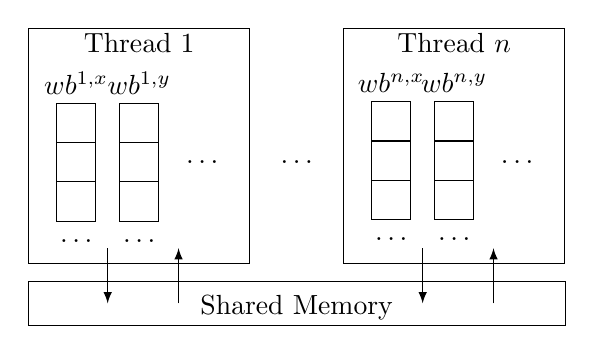
\begin{tikzpicture}
\tikzstyle{wb}=[draw,minimum size=0.5cm]

\begin{scope}[start chain=1 going below,node distance=-0.15mm]
    \node [on chain=1] at (-0.8,11.3) {$wb^{1,x}$};
    \node [on chain=1,wb] {};
    \node [on chain=1,wb] {};
    \node [on chain=1,wb] {};
    \node [on chain=1,wb,draw=none] {$\ldots$};    
\end{scope}

\begin{scope}[start chain=1 going below,node distance=-0.15mm] 
    \node [on chain=1] at (0,11.3) {$wb^{1,y}$} ;
    \node [on chain=1,wb] {};
    \node [on chain=1,wb] {};
    \node [on chain=1,wb] {};
    \node [on chain=1,wb,draw=none] {$\ldots$};    
\end{scope}

\begin{scope}[start chain=1 going below,node distance=-0.15mm] 
    \node [on chain=1,wb,draw=none] at (0.8,10.3) {$\ldots$};   
\end{scope}

\begin{scope}[start chain=1 going below,node distance=-0.15mm] 
    \node [on chain=1,wb,draw=none] at (2,10.3) {$\ldots$};   
\end{scope}        
       
\begin{scope}[start chain=1 going below,node distance=-0.15mm]
    \node [on chain=1] at (3.2,11.3) {$wb^{n,x}$};
    \node [on chain=1,wb] {};
    \node [on chain=1,wb] {};
    \node [on chain=1,wb] {};
    \node [on chain=1,wb,draw=none] {$\ldots$};    
\end{scope}

\begin{scope}[start chain=1 going below,node distance=-0.15mm] 
    \node [on chain=1] at (4,11.3) {$wb^{n,y}$} ;
    \node [on chain=1,wb] {};
    \node [on chain=1,wb] {};
    \node [on chain=1,wb] {};
    \node [on chain=1,wb,draw=none] {$\ldots$};    
\end{scope}

\begin{scope}[start chain=1 going below,node distance=-0.15mm] 
    \node [on chain=1,wb,draw=none] at (4.8,10.3) {$\ldots$};   
\end{scope}

\draw[] node[draw,minimum
        height=85,minimum width=80] (t1) at (0,10.5) {}; 
        \node[anchor=north,inner sep=2pt] at (t1.north)  {Thread 1};
        
\draw[] node[draw,minimum
        height=85,minimum width=80] (t2) at (4,10.5) {}; 
        \node[anchor=north,inner sep=2pt] at (t2.north)  {Thread $n$};
        
 
\draw[] node[draw,minimum
        height=16,minimum width=194] (s1) at (2,8.5) {}; 
        \node[anchor=south,inner sep=2pt] at (s1.south)  {Shared Memory};
        
\draw[-latex] (-0.4,9.2) 	-- (-0.4,8.5)	;
\draw[-latex] (0.5,8.5) 	-- (0.5,9.2)	;

\draw[-latex] (3.6,9.2) 	-- (3.6,8.5)	;
\draw[-latex] (4.5,8.5) 	-- (4.5,9.2)	;
\end{tikzpicture}

\end{document}